\documentclass[a4,center,fleqn]{NAR}

% Enter dates of publication
\copyrightyear{2008}
\pubdate{31 July 2009}
\pubyear{2009}
\jvolume{37}
\jissue{12}

%\articlesubtype{This is the article type (optional)}
\providecommand{\e}[1]{\ensuremath{\times 10^{#1}}}

\begin{document}

\title{\textit{dpcR} a Swiss-army knife for the analysis of digital PCR experiments}

\author{%
Micha\l{} Burdukiewicz\,$^{1,6}$,
Jim Huggett\,$^{2}$,
Alexandra Whale\,$^{2}$,
Bart K.M. Jacobs\,$^{3}$,
Lieven Clement\,$^{3}$,
Piotr Sobczyk\,$^{1}$,
Andrej-Nikolai Spiess\,$^{4}$,
Peter Schierack\,$^{5}$,
Stefan R\"odiger\,$^{5}$\footnote{To whom correspondence should be addressed.
Tel: +49 357385 936; Fax: +49 357385801; Email: stefan.roediger@b-tu.de}}

\address{%
$^{1}$Department of Genomics, Faculty of Biotechnology, University of Wroc\l{}aw, Wroc\l{}aw, Poland
and
$^{2}$Molecular and Cell Biology Team, LGC, Teddington, United Kingdom
and
$^{3}$Department of Applied Mathematics, Computer Science and Statistics, Ghent University, Belgium
and
$^{4}$University Medical Center Hamburg-Eppendorf, Hamburg, Germany
and
$^{5}$Faculty of Natural Sciences, Brandenburg University of Technology Cottbus--Senftenberg, Gro\ss{}enhainer Str. 57, 01968, Senftenberg, Germany
}
% Affiliation must include:
% Department name, institution name, full road and district address,
% state, Zip or postal code, country

\history{%
Received January 1, 2009;
Revised February 1, 2009;
Accepted March 1, 2009}

\maketitle

\begin{abstract}

The digital Polymerase Chain Reaction (dPCR) enables an absolute 
quantification of nucleic acids. Different statistical analysis frameworks
were proposed. However, most analysis is done in closed source software as 
provided by the vendors. This makes it harder to compare results, such as the 
confidence interval estimates. An unified open software framework for 
reproducible research is not available.

To perform dPCR analysis we implemented peer-review statistical methods and 
plots into the \textit{dpcR} framework, based on the sophisticated statistical 
computing environment \textbf{R}. \textit{dpcR} is versatile open source 
cross-platform software framework, which provides functions to process dPCR data 
independent of the hardware. Our software can be used for data analysis and 
presentation, as framework for novel technical developments and as reference for 
statistical methods in dPCR analysis. Features such as functions to estimate the 
underlying Poisson process, calculation of confidence intervals based on single 
samples as well as on replicates, a novel Generalized Linear Model-based 
procedure to compare dPCR experiments and a spatial randomness test for 
assessing plate effects have been integrated. We use a plug-in like architecture 
and abstraction layers to make the framework usable for droplets and (real-time) 
chamber based technologies.

\textit{dpcR} is implemented with interfaces to the command-line, graphical 
user interfaces and interactive web application. Therefore, it can be used by 
novices in a graphical user interface or by experts via a command-line 
interface. The \textit{dpcR} framework can be used to build a custom-made 
analyser according to the user requirements. \textit{dpcR} is an 
open framework, which can be easily adapted to the growing knowledge in dPCR. 
  
\end{abstract}


\section{Introduction}

The digital PCR (dPCR) is an important contender for precise nucleic acids 
quantifications. Application of the dPCR include investigation of allele 
frequencies, single-cell analysis, gene expression analysis and absolute quantification of PCR 
products. The chemical basis (e.g., buffer, primer) of the dPCR and thermal 
cycling is similar to the real-time quantitative qPCR (qPCR). Though, approaches 
based on isothermal amplification were also developed 
\cite{pabinger_survey_2014, ludlow_2014, rodiger_r_2015}. A first proposal for a 
dPCR-like approach and the use of the Poisson distribution to quantify the 
number of molecules on a ``sample'' was shown by Ruano \textit{et al.} 1990 
(PNAS) with the single molecule dilution (SMD) PCR \cite{ruano_haplotype_1990}. 
In 1999 Vogelstein \textit{et al.} (PNAS) described the first true dPCR 
\cite{vogelstein_digital_1999}. In contrast to qPCR, the amplification reaction 
does not take place in a single reaction chamber. Rather its a process of clonal 
amplification in small separate ``partitions'' (e.g., nl volume droplets of 
water oil emulsions, chambers on micro structured chips). The number of positive 
partition in relation to the number of total partitions. By applying Poisson 
statistics it is possible to determine the number of the starting material in 
given volume. Therefore, the dPCR does not require an external calibration. Since approximately ten years the 
dPCR is gaining momentum in the mainstream user-base and will likely have the 
same impact as the qPCR methodology. There is an intensive research on dPCR 
platforms with the overall aim to make to technology broadly usable, cheap, 
robust and to enable high sample throughput \cite{selck_increased_2013, huggett_qpcr_2015, 
morley_digital_2014, rodiger_r_2015}.

% **************************************************************
% Keep this command to avoid text of first page running into the
% first page footnotes
\enlargethispage{-65.1pt}
% **************************************************************
  
The dPCR has some principle assumptions and fundamental properties. First of all 
the chemical reaction should be unaffected by inhibitors. The distribution of 
the single molecule target regions follows a Poission distribution. The Poisson 
distribution appears like a normal distribution but without negative values and 
being zero the lowest. First, a large number (n) of amplifications reactions as 
required to have a high statistical power. Therefore, a high number of PCR 
reactions is needed. For Poisson distributions an n of XY (get reference from 
table/text book form statistics/biostatistics?) is considered large. Second, that 
the molecules required for the amplification amplifications reactions are 
randomly distributed in the compartments. Visual analysis and statistical 
analysis can be used to test for randomness of the reaction and thus to exclude 
the clustering of of positive reactions \cite{Baddeley_2015}. A 
clustering of positive wells might be due to sample loading or analysis process 
(systematic error). The outcome of an amplification can be no amplification 
(less than 1 target copy per volume), an unsaturated reaction with a 
binary/``multinary'' amplification (usable to calculate the ``concentration'') 
or a saturated reaction where virtually all compartments are positive.

Chambers or emulsion based droplets are the dominant technical approaches to 
create partitions for dPCR  reactions \cite{morley_digital_2014}. However, other 
approaches based on beads were shown too \cite{shuga_single_2013}. Chamber based dPCR 
systems have fixed geometries, including the volume of the reaction chambers. 
Despite the fact that dPCRs is an endpoint analysis the chamber based 
technologies allow generally the real-time monitoring of the amplification 
reaction and subsequent confirmation of the amplification reaction be melting 
curve analysis \cite{mojtahedi_2014}. Thus, such technologies enable easier 
trouble shooting and quality management of the data. However, the downside of 
these technologies is the fixed limited number of compartments and the price. 
The emulsion based dPCRs are easier to perform since the compartments are 
generated by microfluidic technologies and have practically no limitation 
regarding the number of compartments. This results in a higher statistical power 
to quantify small differences in sample quantities. The emulsion chambers are 
made of water-in-oil emulsions with similar sizes.

There is a need for an vendor independent data analysis. For example, others 
have written custom made scripts for data analysis in \textbf{Mathematica} 
(Wolfram Research), \textbf{MS EXCEL} (Microsoft) or \textbf{R} 
\cite{strain_highly_2013, dreo_optimising_2014, trypsteen_ddpcrquant_2015, 
dobnik_multiplex_2015}. Recently, Mathew \textit{et al.} published the open 
access bioinformatic pipeline, designated \textbf{definetherain} 
\cite{jones_low_2014}. The tool is coded in JavaScript and has been made 
available for free in a web browser. However, this is of limited use, since the 
solutions are tied to the droplet dPCR by Bio-Rad, 
operating system platform for data analysis and only usable for a single task. 
Moreover, we found no software packages with GUIs and bindings to a 
sophisticated statistical computing environment for reproducible research. 

% **************************************************************
% Keep this command to avoid text of first page running into the
% first page footnotes
%\enlargethispage{-65.1pt}
% **************************************************************
In 2013 we started the developmen of the \textit{dpcR} framework to perform 
analysis of dPCR experiments for \textbf{R} software 
\citep{burdukiewicz_dpcr:_2013}. R is widely used for statistical analysis of 
biomedical data and is freely available for the MacOS, Linux/Unix and Windows 
operating systems. \textit{dpcR}  may be used in conjunction with literate 
programming \textbf{R} packages (e.g., \textit{knitR}) and tools for 
reproducible research (e.g.,  \textit{rctrack}) \cite{liu_r_2014, 
rodiger_r_2015}. 

\section{MATERIALS AND METHODS}

\subsection{Implementation}

We have chosen \textbf{R} because it is cross-platform and the \textit{lingua 
franca} in applied statistical bioinformatics. Since all software is open source 
it is possible to track numerical errors \cite{rodiger_rkward_2012, 
rodiger_r_2015}. Most \textbf{R} packages depend on other packages 
\cite{ooms_2013}. The same holds true for \textit{dpcR}. This results in a 
complex network of recursive dependencies (Figure~\ref{dpcR_framework}A). Core 
packages include \textit{qpcR} \cite{ritz_qpcr_2008}, \textit{shiny}, 
\textit{MBmca} \cite{rodiger_surface_2013}, \textit{chipPCR} 
\cite{roediger2015chippcr}. A basic design decision was to structure specific 
properties of dPCR systems (droplet vs. chamber) in auxiliary functions. Selected 
chamber dPCR systems rely on the proper preprocessing of qPCR data. This 
functionality is inherited from the \textit{qpcR} \textbf{R} package.

The naming convention of \textit{dpcR} is \texttt{underscore\_sep} 
\cite{Baaaath_2012}. The main \textit{dpcR} functions (e.g., for analysis, 
simulations, plotting), several auxiliary functions (e.g., data import) and 
datasets of different dPCR systems are shown in the workflow of Figure 
\ref{workflow}. Figure~\ref{dpcR_framework}B illustrates the implementation of 
the \textit{dpcR} package. The function \textit{read\_dpcr}, \textit{qpcr2pp} 
and \textit{sim\_dpcr}, sets the input for all objects in the \texttt{dpcr} 
class. Central calculation specific to Poisson statistics in are performed 
independently in main functions. This class manages details of the dPCR analysis 
that are subsequently processed by \textit{dpcR} functions (e.g., 
reading/writing). Further details are explained in the supplementary 
information.

\begin{figure*}[t]
\begin{center}
\includegraphics[page = 2, trim = 0cm 1cm 0cm 0cm, clip, width=17cm]{dpcR_analysis.pdf}
\end{center}
\caption{Implementation of the \textit{dpcR} package. \textbf{(B)} Modular software 
framework structure. \textit{dpcR} is typically run from a desktop computer or a 
server. The software can be operated by an GUI/IDE application such as 
\textbf{RStudio} or \textbf{RKWard}. The \textit{dpcR} package has dependencies 
to other \textbf{R} packages (middle layer). The functionality shared between 
the packages enables repaid addition and expansion of functionality.}
\label{dpcR_framework}
\end{figure*}

\begin{figure*}[t]
\begin{center}
\includegraphics[page = 1, trim = 0cm 10cm 0cm 0cm, clip, width=17cm]{dpcR_analysis.pdf}
\end{center}
\caption{\textit{dpcR} workflow. The diagram shows main functions 
available at each step of a dPCR data analysis.}
\label{workflow}
\end{figure*}

Figure~\ref{workflow} provides an overview of important functions available at 
each step of a dPCR analysis. The first step is to import sample data into the 
\textbf{R} session. \textit{dpcR} accepts various data structures. This includes 
matrices of raw data and predefined structures provided by the different vendors 
(see Table \ref{table_formats}). Moreover, \textit{dpcR} accepts objects from 
the \textbf{R} workspace, which are converted via the \textit{read\_dpcr} 
function. Novel raw data structures are processed outside \textit{dpcR} using 
tools as described elsewhere. The data input to \textit{dpcR} should be raw data 
preferable, rather than gated summary data. The reasoning it to keep control 
over information loss for reproducible research.

\subsection{Documentation}

All functions of the \textit{dpcR} package have its own documentation package, 
which specifies the input types, classes, parameters and output formats. The 
documentation is available as standard \textbf{R} package reference manual and 
as vignette.

According to the dMIQE guidelines \cite{huggett_digital_2013} we used following notation:

\begin{itemize}
 \item $\lambda$: average molecule numbers per partition,
 \item $k$: number of molecules per partition,
 \item $m$: total number of the molecules.
\end{itemize}

The following convention was kept, both in the documentation and in the 
package source code.

\subsection{Import and export of results figures and data}

\subsubsection{Reading or importing data}

\textbf{R} has a rich set of tool to arrange data in order to prepare them for 
the analysis. This is important when it comes to the question how experiments 
should be treated \citep{rodiger_r_2015}.

Most \textit{dpcR} import functions take a data matrix of annotated numeric 
(e.g, fluorescence amplitude) and integer values (e.g., counts) as input. The 
\textit{raw\_data} input was implemented  make data input easier for the end 
user (see Supplement). Such input files can be manually created in a spreadsheet 
program or text editor.

There numerous methods to import amplification curve data into the \textbf{R} 
workspace \cite{perkins_readqpcr_2012, pabinger_survey_2014, rodiger_r_2015}. 
Prior processing the data for dPCR analysis it is recommended to use dedicated 
\textbf{R} packages, such as \textit{chipPCR} \cite{roediger2015chippcr}, 
\textit{MBmca} \cite{rodiger_surface_2013}, \textit{qpcR} \cite{ritz_qpcr_2008}, 
to pre-process (e.g., removal of missing values, smoothing 
\cite{spiess_impact_2015}) the raw data.

(see Table \ref{table_formats}).

\begin{table}[b]
\tableparts{%
\caption{Structured vendor export data formats handled by \textit{dpcR}~v.~0.5 and later.}
\label{table_formats}%
}{%
\begin{tabular*}{\columnwidth}{@{}llll@{}}
\toprule
Vendor & System & Format & Type
\\
\colrule
Bio-Rad & QX100 \& QX200 & CSV & Summary export
\\
Fluidigm & BioMark & CSV & Summary export
\\
Formulatrix & Constellation Digital PCR & CSV & Summary export
\\
\botrule
\end{tabular*}%
} {The number of structured export data formats handled by \textit{dpcR} is 
growing. Numerous data formats can be processed with the functionality provided 
by the \textbf{R} environment (see \cite{rodiger_r_2015}). CSV, comma separated 
values.}
\end{table}

\subsubsection{\textit{De novo} creation of dpcR objects from raw data}

In experimental setups user have the need to transform their raw data in a 
processable format. Since the \textbf{R} environment is cross-platform an 
ubiquitously used we aimed to ease this creation. In particular, this is 
relevant for reproducible research. The \textit{dpcR} framework covers the types 
typically used in laboratories.

\subsubsection{Public data sets}

\textit{dpcR} includes data sets or refers to additional R packages for testing 
purposes. The data originate from different dPCR and qPCR systems and were 
either published previously \cite{whale_comparison_2012, roediger2015chippcr, 
white_digital_2009, rodiger_r_2015} or \textit{de novo} generated.

\subsubsection{Export of analysis results}

Since \textit{dpcR} is based on the \textbf{R} environment all facilities for a 
report generation are usable as described before \cite{rodiger_r_2015}.

(see Table \ref{table_formats}).

A commonly available data exchange format is a perquisite for reproducible 
research. So far no cross-platform and system-independent format has been 
introduced for dPCR experiments. Therefore, we decided to use \texttt{RData} as 
our default format. \texttt{RData} works across all \textbf{R} environments and 
saves the variable names along the content of multiple variables, which can be 
restored in any workspace.

\subsection{Calculation of the uncertainty}

To determine the uncertainty of the estimated $\lambda$ we employ two previously 
published peer-reviewed methods \cite{dube_mathematical_2008, bhat_single_2009}.

$PUTDUBEANDBHATEQUATIONSHERE$

\subsection{Poisson distribution}


\subsubsection{Moments}
It is assumed that results from the dPCR reaction follow the Poisson 
distribution. We implemented several functions for computation of the four first 
moments (mean, variance, skewness, kurtosis) of the distribution from which the 
data is sampled. They can be calculated empirically from the sample data or as 
functions of the estimated $\lambda$.

\subsubsection{Binomial approximation}
Since dPCR data contain binarized Poisson 
counts (all counts than zero are grouped together) it is possible to use methods 
appropriate for Binomial distribution. We employ several methods of computing 
confidence intervals (CI) for $\lambda$ value (e.g., Wilson method, 
Agresti-Coull method). They especially advantageous when $k$ is considerably 
smaller than $m$. They are beneficial for uncertainty calculation, because 
yielded CI's are not oscillating in such scenarios \cite{brown_2001}.

\subsection{Simulation}

The package covers two Simulation methods as described elsewhere in 
peer-reviewed publications. The method proposed by Dube~\textit{et al.}~2008 
\cite{dube_mathematical_2008} is based on distributing template molecules over 
partitions. The procedure in Jacobs~\textit{et al.}~2014 \cite{jacobs_2014} is 
more sophisticated and returns the fluorescence value obtains from droplet dPCR 
experiment including such phenomena as ``rain''. We also added streamlined and 
high-performing simulation in assumptions similar to Dube~\textit{et al.}~2008.

\subsection{Comparison of dPCR experiments}

In \cite{Burdukiewicz_tba} We implemented statistics based on Generalized Linear Models (GLM) and 
\textit{multiple ratio testing} (\textit{MRT}) to compare dPCR experiments. 

\subsection{Spatial distribution}

Array based dPCR experiments provide information about spatial distribution of 
partitions. Procedures belonging to spatial statistics verify if the status 
(positive, negative) of partition depends on its location. To address such 
questions, we implemented a Complete Spatial Randomness test for dPCR arrays. 
Moreover, we provide functionalities to export array dPCR data to \textbf{R} 
packages specialized in spatial statistics as described in 
\cite{Baddeley_2015}.

\subsection{Converting qPCRs to dPCRs}

High-Throughput qPCR is a well established and robust technology, which allows 
precise quantification of DNA material in high throughput fashion. However, the 
quantification by qPCR is challenging at very low and very high concentrations. 
In addition, pre-processing and data analysis is a affected by numerous adverse 
effects \cite{ruijter_2013, pabinger_survey_2014, spiess_impact_2015}. But the 
amplification curve real-time monitoring of the PCR product formation enables to 
determine quantification points (Cq), which can be binarized and analysed in the 
same way as dPCR experiments \cite{mojtahedi_2014}. This functionality is 
integral part of the \textit{dpcR} package.

Figure\ref{qpcr2pp_1}

\begin{figure}[t]
\begin{center}
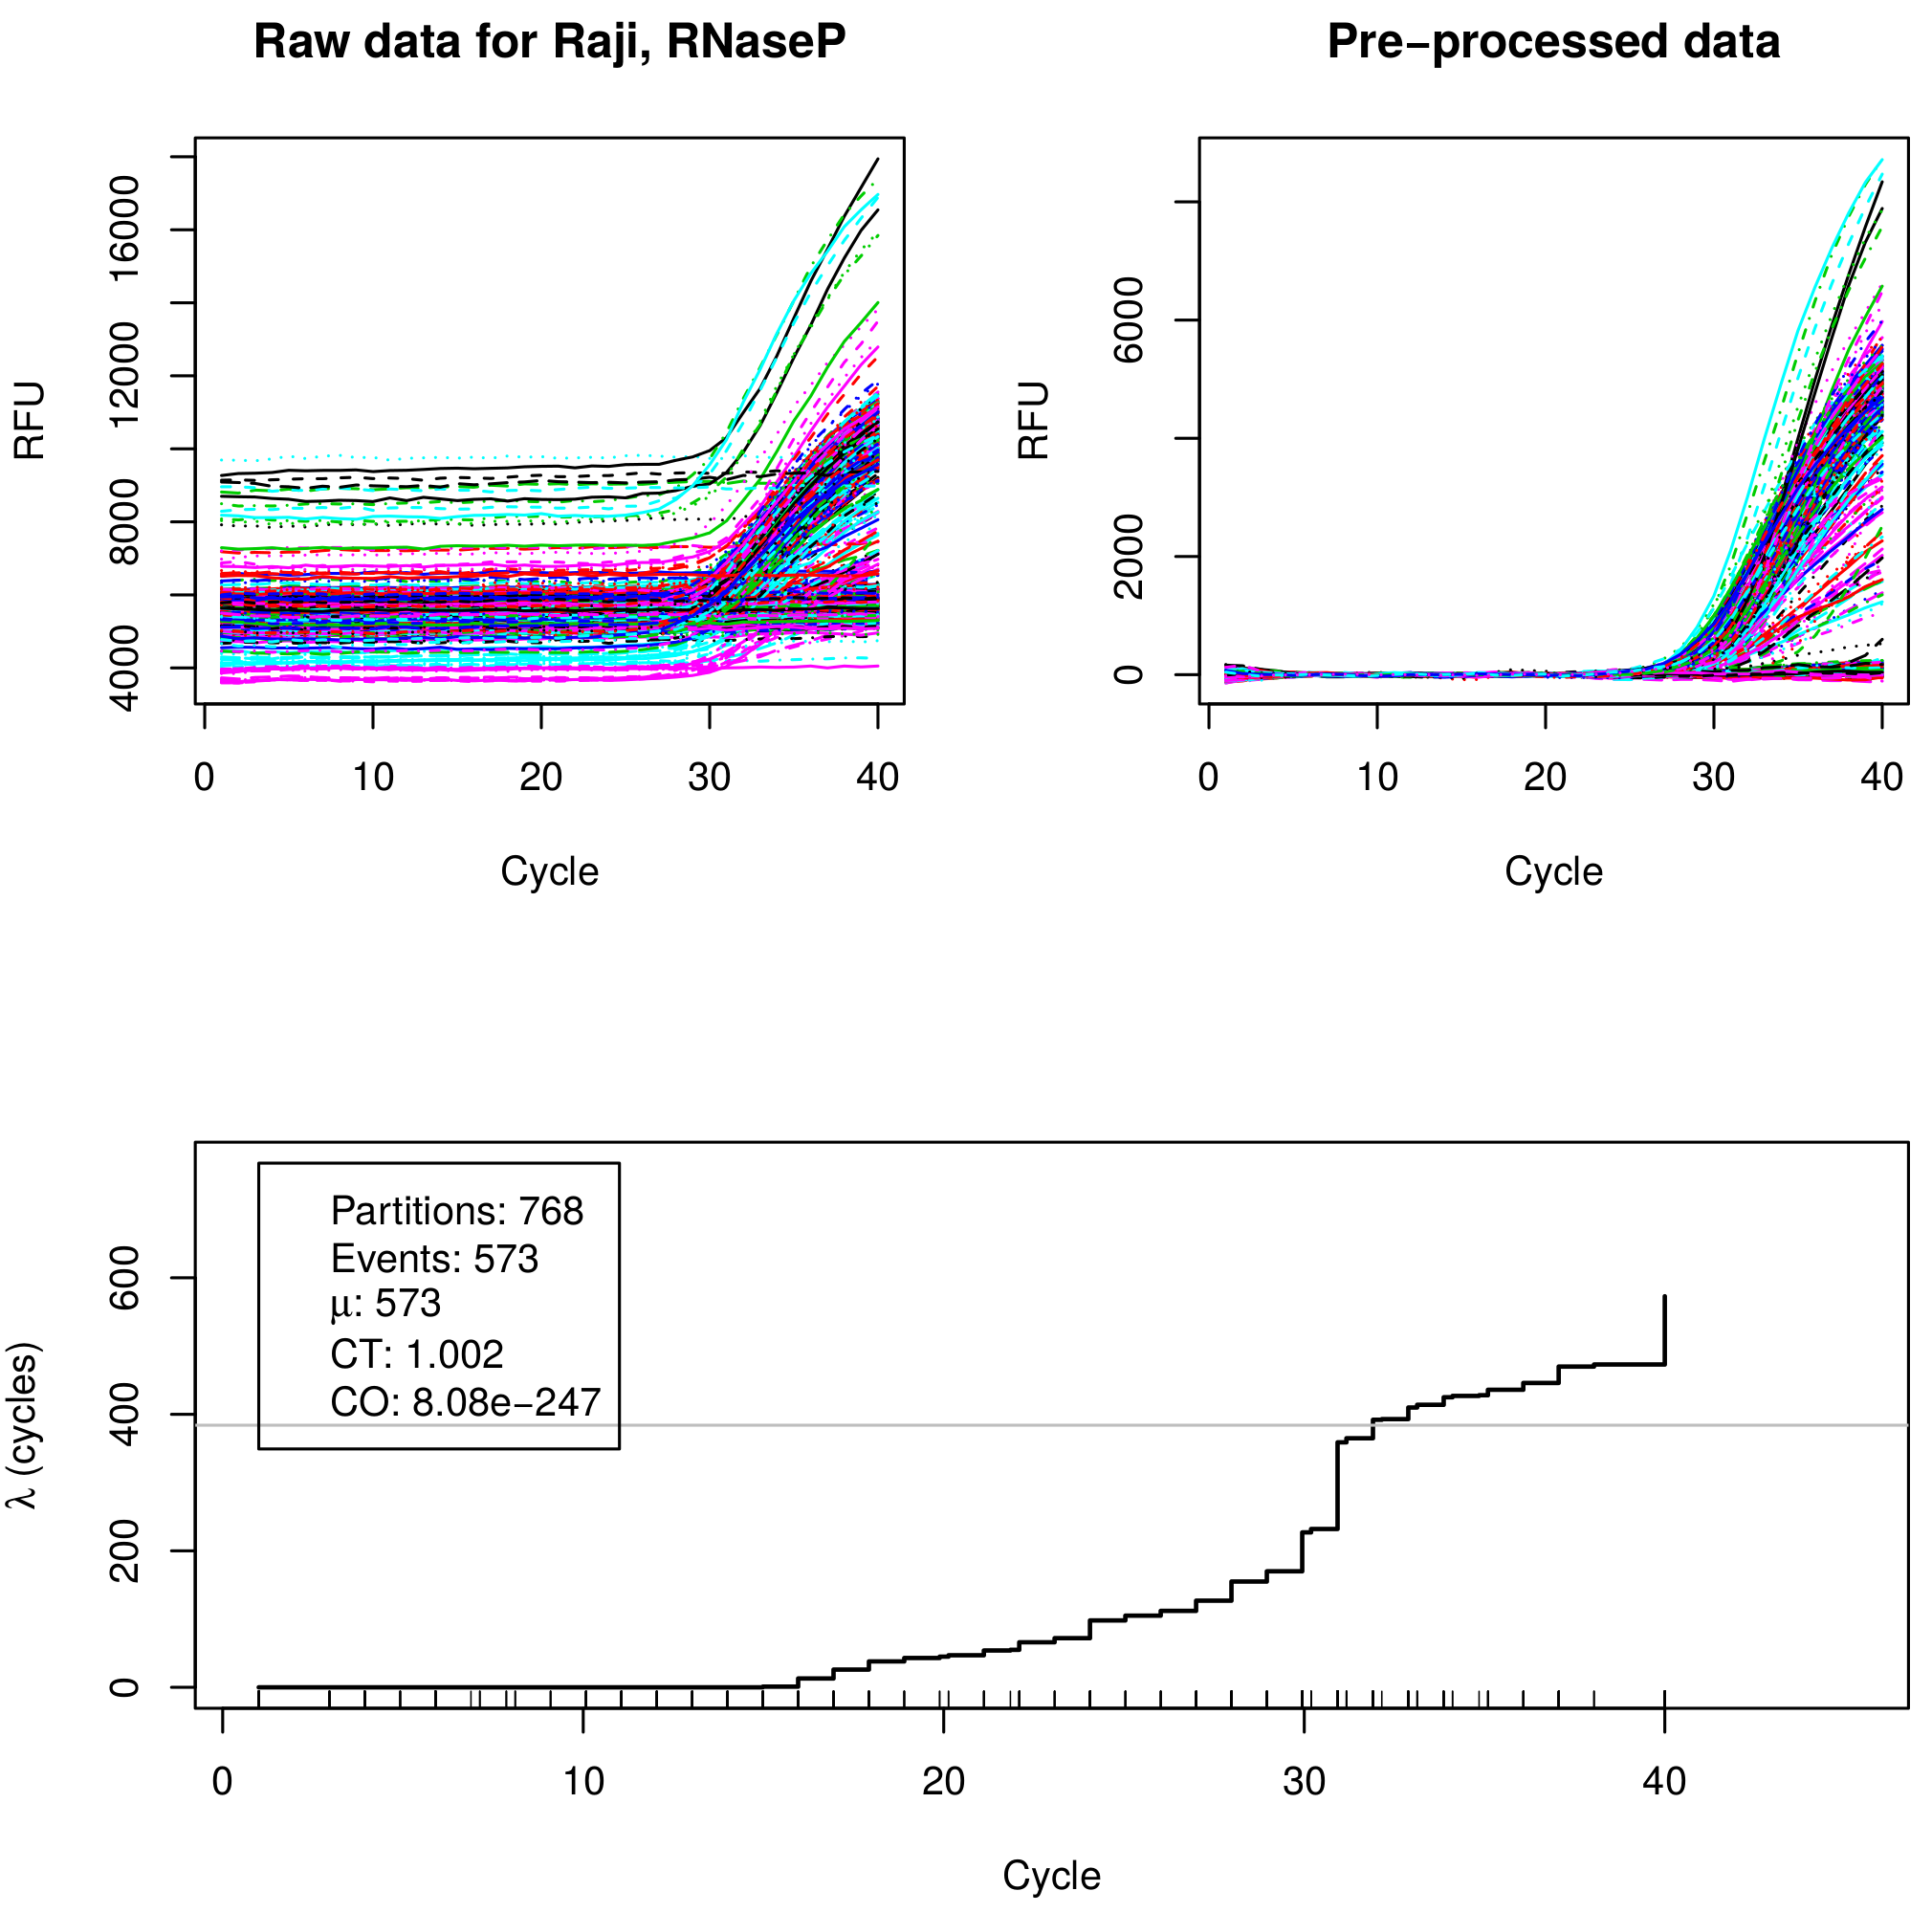
\includegraphics[width=9cm]{qpcr2pp_1.png}
\end{center}
\caption{Uncover characteristics of dPCR data. 
Selected dPCR platforms are qPCR platforms at the same time. The function \textit{qpcr2pp} uses the 
qPCR amplification curve data and interprets them as dPCR (Poisson process). A) Raw data of The 
function were B) preprocessed (baselined, smoothed) with functions from the 
\textit{chipPCR} package and C) finally analysed (Cq calculation $\rightarrow$ binarize) with the 
\textit{qpcr2pp} (qPCR to Poisson process) function from the \textit{dpcR} package.} 
\label{qpcr2pp_1}
\end{figure}

\section{RESULTS}

In the following section we show applications of the \textit{dpcR} package.

\subsection{Evaluation of dPCR comparison methods}

TBD

\subsection{Graphical user interface}

The critical functionalities of \textit{dpcR} package are implemented in the 
\textit{dpcReport} GUI. We aimed for a form factor (e.g., smart phone, tablet, 
desktop PCR) and operating system independent implementation of a graphical user 
interface. \textit{dpcReport} is based on \textit{shiny} technology and offers 
an intuitive user interface, which can be accessed by browsers (e.g., Google 
Chrome, Mozilla Firefox). The advanced plots are based on \textit{ggplot2} (see Supplement).

The first panel ``Input file'' is responsible for loading the input data. Here 
part of data input structure (e.g., ID of experiments) may be accessed and 
modified during the analysis in the GUI. The second panel ``Data summary'' 
presents descriptive summary of the data in form of interactive tables and 
plots, offering filtering and selecting of individual runs. The third panel 
``Comparison of runs'' compares all runs of the experiment data. The fourth 
panel ``Advanced analysis'' consists of more specialized functionalities as 
testing individual arrays. All statistical methods used in the GUI are integral 
part of the \textit{dpcR} package and described in the methods section. The last 
panel enables flexible report generation. The report can be customized by 
including various sections, which are equivalents of the GUI panels.

An interesting feature of the \textit{shiny} 
technology is the automatic integration in environments, which support 
\texttt{HTML5} and \texttt{ECMAScript}. The \textit{dpcReport} integrates into 
Integration in third party software. This can be a modern web~browser or an 
\textbf{R} IDE/GUI such as \textbf{RKWard} (Figure~\ref{GUI_RKWard_1}) 
\cite{rodiger_rkward_2012} or \textbf{RStudio}. \textit{dpcReport} is a GUI tool 
for dPCR data mining and report generation. User can interact via a 
point-and-click interface on different tabs, which contain widgets such as 
sliders, input fields and check boxes. Other 
user input, such as parameters of test performed in GUI, are preserved and 
returned in the report to increase the reproducibility of the research study. 
The tabs cover relevant analysis steps for the report generation. An important 
option of \textit{dpcReport} is an export of the \textbf{R} source code used for 
the report generation is provided to the user. This code can be used for 
recreating the analysis in the \textbf{R} environment or prototyping more 
complicated workflows.


\begin{figure*}[t]
\begin{center}
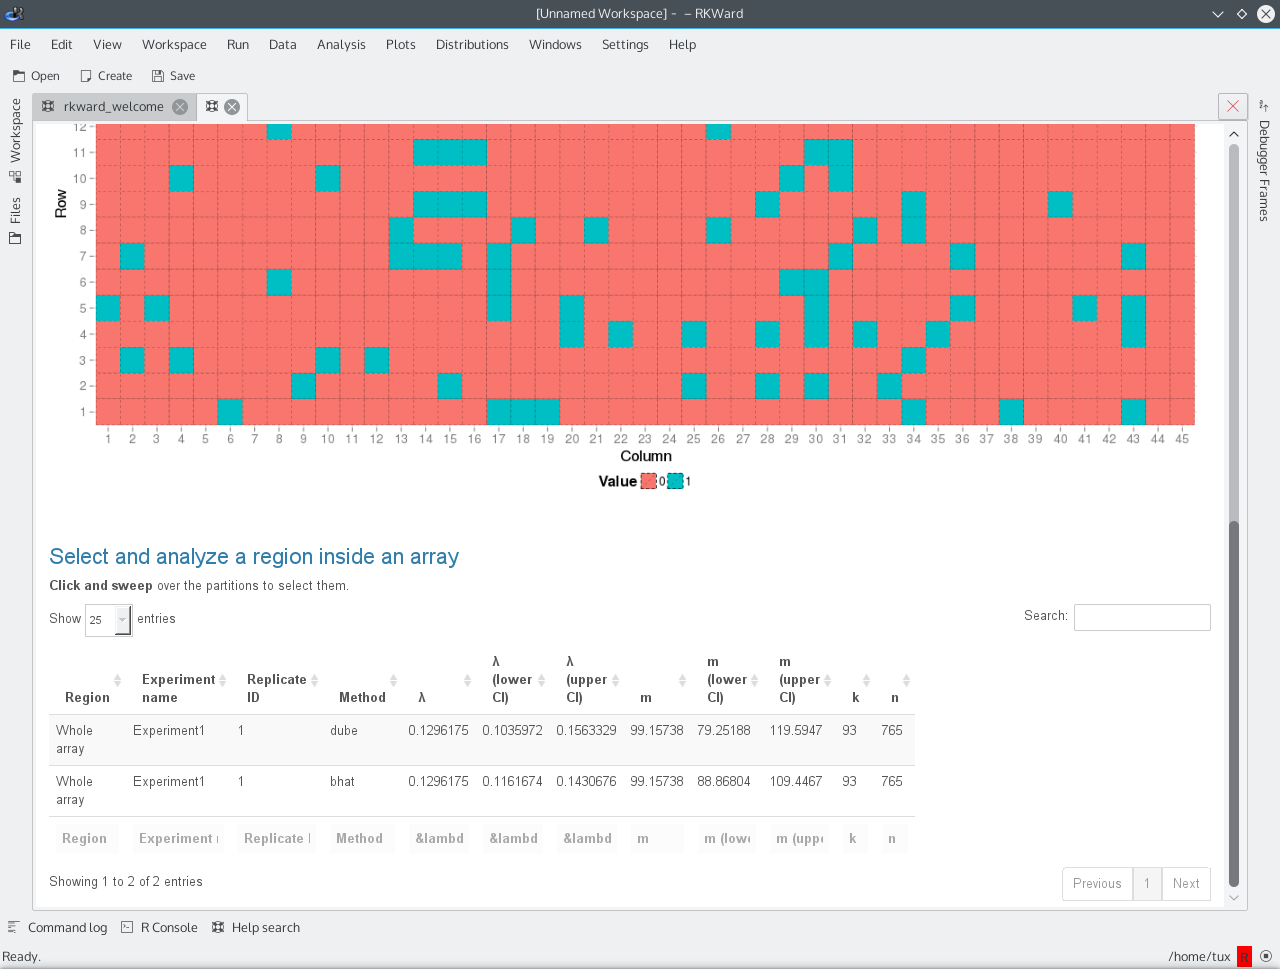
\includegraphics[width=17cm]{GUI_RKWard_1.png}
\end{center}
\caption{\textit{dpcReport()} function running in the graphical user interface and integrated development environment \textbf{RKWard}.}
\label{GUI_RKWard_1}
\end{figure*}

\subsection{Vendor independent data analysis}

QX100 series is no longer available. Instead, the newer version QX200
protocol
consisting of the QX200 droplet generator (Bio-Rad, cat. no. 186-4002) and
the QX200 droplet reader (Bio-Rad, cat. no. 186-4003) can be purchased,
for which the protocol can be applied without changes. Alternative dPCR
devices available from, e.g., RainDance Technologies, Life Technologies or
JN Medsys \citep{mock_digital_2016}.

\subsection{Automatic report generation}

In \cite{rodiger_r_2015} we gave an example where we re-analyze droplet dPCR 
data from a Bio-Rad QX100 system with an early implementation of the 
\textit{dpcR} package. As recommended in the dMIQE guidelines 
\cite{huggett_digital_2013} we included key elements in the report.
\subsection{Availability}

The \textit{dpcR} framework is available as open source software package (GPL-3 
or later) as part of the Bioconductor project \cite{gentleman_2004}. The stable 
version is hosted at http://cran.r-project.org/web/packages/dpcR and the source 
code is available from  https://github.com/michbur/dpcR.

\section{DISCUSSION}

Currently, there exist different dPCR analysis software solutions provided by 
the vendors. But most of the software packages are black boxes, which 
prevent deep insight into the data processing step. Other and we think that 
scientific software should be open \cite{ince_case_2012, 
rodiger_r_2015}. In addition, most of the software solutions are aimed to be 
used in very specific scenarios and a mutual exclusive to alternative platforms 
(e.g., droplet vs. chamber-based). We have chosen \textbf{R} because it is the 
\textit{lingua franca} in biostatistics and broadly used in other disciplines 
\cite{rodiger_r_2015}. We developed the \textit{dpcR} package, which is a 
software framework for analysis of dPCR. \textit{dpcR} provides the scientific 
community a broadly applicable tool for teaching purposes, data analysis and 
theoretical research based on simulations. Our software framework can be used to 
accelerate the development of new approaches to dPCR.

Functions included may be used to simulate dPCRs, perform statistical data 
analysis, plotting of the results and simple report generation. 

\section{CONCLUSION}

In conclusion, \textit{dpcR} provides means to understand how dPCR works, 
to design, simulate and analyze experiments, and to verify their results (e.g., 
confidence interval estimation), which should ultimately improve 
reproducibility. We have built what we believe to be the first unified, 
cross-platform, dMIQE compliant, open source software framework for 
analysing dPCR experiments. Our \textit{dpcR} framework is 
targeted at a broad user base including end users in clinics, academics, 
developers, and educators. We implemented existing statistical methods for dPCR 
and suggest the introduction of a standardized dPCR nomenclature. Our 
framework is suitable for teaching and includes references for an elaborated 
set of methods for dPCR statistics. Our software can be used for (I) data 
analysis and visualization in research, (II) as software framework for novel 
technical developments, (III) as platform for teaching this new technology and 
(IV) as reference for statistical methods with a standardized nomenclature for 
dPCR experiments. The framework enables the simulations and predictions of Poisson 
distribution for dPCR scenarios, the analysis of previously run dPCRs. Due to 
the plug-in structure of the software it is possible to build custom-made 
analysers.

We decided not to implement algorithms for clustering and ``rain'' (positive 
droplets) definition of droplet dPCR data. This is because, there are several 
\textbf{R} packages from flow-cytometer research. Implementations range from 
manual to automatic clustering \cite{le_meur_computational_2013, milbury_determining_2014, Malek15022015, 
trypsteen_ddpcrquant_2015}. Moreover, discussion with our peers and the 
literature suggest that a consensus of an appropriate method for dPCR is not 
available \cite{trypsteen_ddpcrquant_2015}.

Our open framework includes to invitation to the scientific community to join and 
support the development of \textit{dpcR}.


\section{ACKNOWLEDGEMENTS}

Grateful thanks belong to the \textbf{R} community and the \textbf{RStudio} developers.

\section{Funding}
This work was funded by the Federal Ministry of Education and Research (BMBF) InnoProfile--Transfer--Projekt 03 IPT 611X.
 
\subsubsection{Conflict of interest statement.} None declared.
%\newpage

\bibliographystyle{plain}
\bibliography{dpcr}
\end{document}
